In this chapter, we analyze the first experiment, that is, the impact of using different consensus algorithms in a Blockchain-based Federated Learning system. In this set of experiments, all properties of the system are static, except for the consensus algorithm, which varies between PoA, PoW and QBFT.

\section{Execution Time, Transaction Cost and Latency}

The first interesting statistics we look into are the E2E time, the mean time it takes for a round to complete, as well as the mean transaction latency and the mean transaction cost. These are represented in \autoref{tab:metrics_consensus_algorithms}.

\begin{table}[!ht]
\centering
\begin{tabular}{c|c|c|c} \hline \hline
Metric                              & PoA    & PoW    & QBFT   \\ \hline \hline
E2E Time (m)            & 18.93  & 30.62  & 18.97  \\ \hline
Mean Round Time (s)             & 22.70  & 36.72  & 22.74  \\ \hline
% Median Time Per Round (s)           & 21.90  & 35.28  & 21.99  \\ \hline \hline
Mean Transaction Latency (s)    & 1.549  & 1.821  & 1.558  \\ \hline
% Median Latency Per Transaction (s)  & 1.549  & 1.554  & 1.555  \\ \hline \hline
Mean Transaction Cost (Gas)     & 183124 & 227052 & 182880 \\ \hline
% Median Cost Per Transaction (Gas)   & 185198 & 229866 & 185068 \\ \hline \hline
\end{tabular}
\caption{Time and Transaction Metrics Per Consensus Algorithm}
\label{tab:metrics_consensus_algorithms}
\end{table}

Regarding time, we can observe that different consensus algorithms can lead to very different running times. On one hand, PoA and QBFT are the fastest consensus algorithms, providing the lowest E2E times and mean round times. Additionally, the difference between both is minimal, differing only $0.04$ seconds per round. On the other hand, PoW takes the longest, being $1.6$ times slower than both PoA and QBFT.

Transaction latency and costs follow a similar trend as the running times. Both PoA and QBFT have similar transaction latency and cost, differing in a small amount, while PoW has a higher transaction latency and cost. When compared, PoW costs $1.2$ times more than using PoA and QBFT.

As explained in \autoref{background:consensus_algorithms}, PoW works by solving increasingly complex mathematical puzzles that consume high amounts of resources. This intense process can lead to slower response rates, which translates to higher transaction latency and costs. This, in turn, increases the time it takes for each round to complete.

\section{Accuracy}

Regarding accuracy, as can be seen in \autoref{fig:accuracy_consensus_algorithms}, it does not change significantly with different consensus algorithms. Consensus algorithms dictate the order at which the transactions are processed and ensures consistency between the multiple blockchain nodes. This only affects the blockchain inner workings, and not the ML process. Therefore, it was not expected that the consensus algorithms would have an impact on the accuracy.

\begin{figure}[!ht]
    \centering
    \centering
    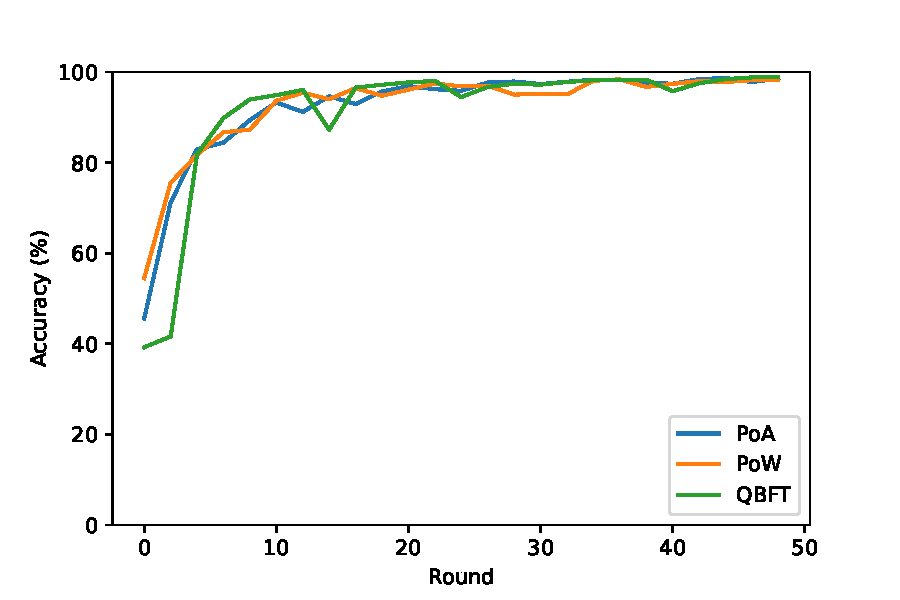
\includegraphics[width=0.7\textwidth]{graphics/01_consensus_accuracy.pdf}
    \caption{Accuracy Per Consensus Algorithm}
    \label{fig:accuracy_consensus_algorithms}
\end{figure}

\section{Communication Costs}

For the communication costs, we analyze the inbound and outbound network traffic per round at the training clients, computing servers and blockchain nodes. This values can be observed in \autoref{fig:net_consensus_algorithms}.

On one hand, the inbound and outbound traffic for the clients and server has negligible differences when using different consensus algorithms. As mentioned in the previous section, the consensus algorithms have no expected impact on the ML process. Since the clients and servers only concern the ML process, it was expected that the clients and servers would not be affected. The small differences we can observe, in the order of $< 2$ MB, are likely connected to fluctuations in the random participant selection technique. If there are more participants being selected, more data needs to be transmitted, and vice-versa.

On the other hand, the traffic at the blockchain nodes varies considerably depending on the consensus algorithm. On average, PoW requires more bandwidth per round than PoA, but the difference is very minimal. However, QBFT requires $2$ times more network traffic than PoW and $4$ times more traffic than PoA. QBFT is a three-phase consensus algorithm, which requires a higher amount of network messages to be transmitted before reaching consensus. In addition, the size of the messages also differs. When combining both of this aspects, we can conclude that the expected network traffic per round using the QBFT algorithm would be higher.

\begin{figure}[!ht]
    \centering
    \centering
    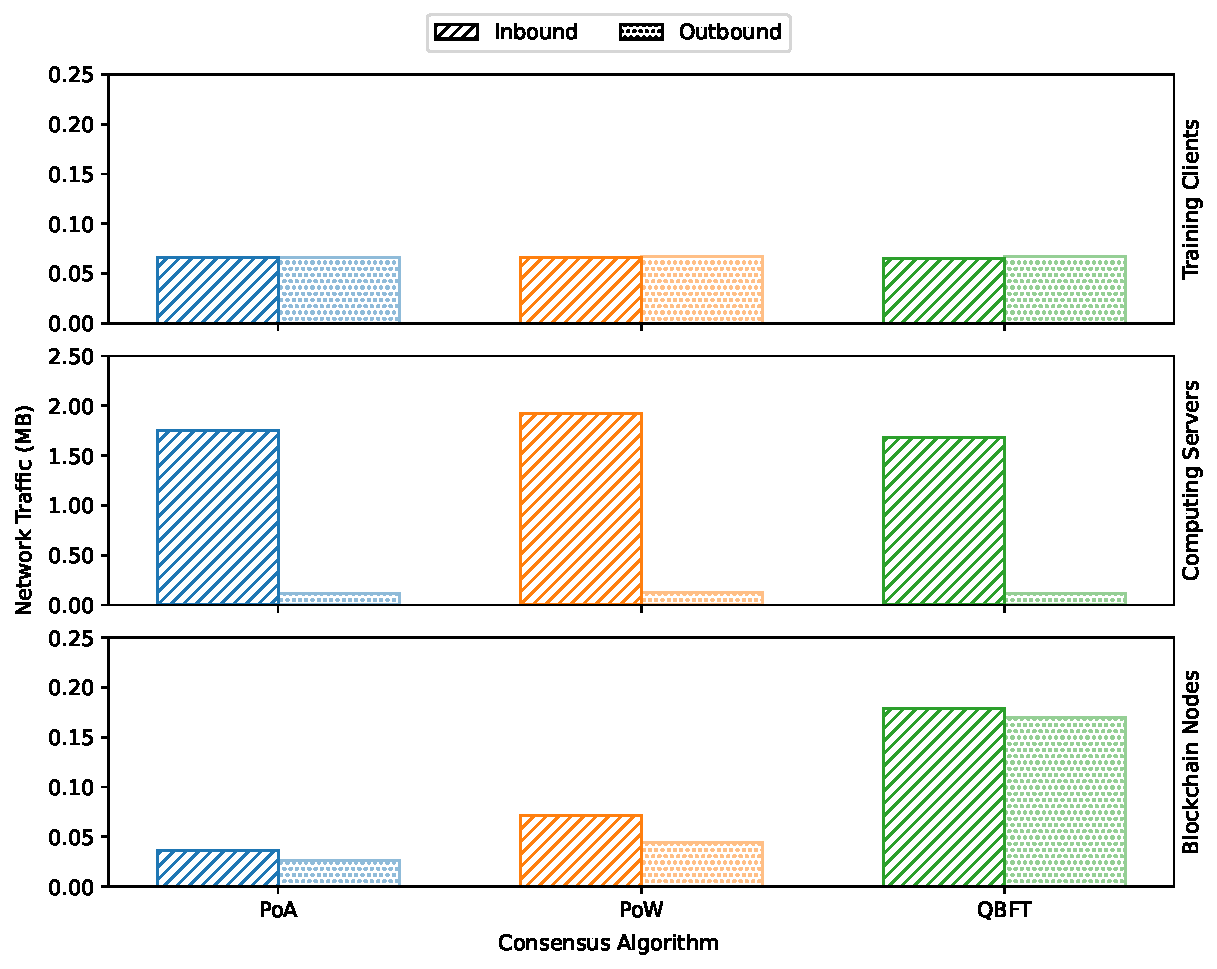
\includegraphics[width=0.8\textwidth]{graphics/01_consensus_net.pdf}
    \caption{Network Traffic Per Round Per Consensus Algorithm}
    \label{fig:net_consensus_algorithms}
\end{figure}

\section{Computation Costs}

Regarding computation costs, we will look at both RAM and CPU usage on the training clients, computing servers and blockchain nodes. To do so, we have \autoref{fig:ram_consensus_algorithms} and \autoref{fig:cpu_consensus_algorithms}, that show the mean RAM usage and mean CPU usage, respectively, per consensus algorithm during the execution of the experiments. As mentioned previously, the execution times for PoA and QBFT are lower than for PoW, which can be seen in the figures by not having more data past minute 19. Additionally, as explained before, the consensus algorithms are not expected to have a direct impact on the clients or the servers.

\begin{figure}[!hpt]
    \centering
    \centering
    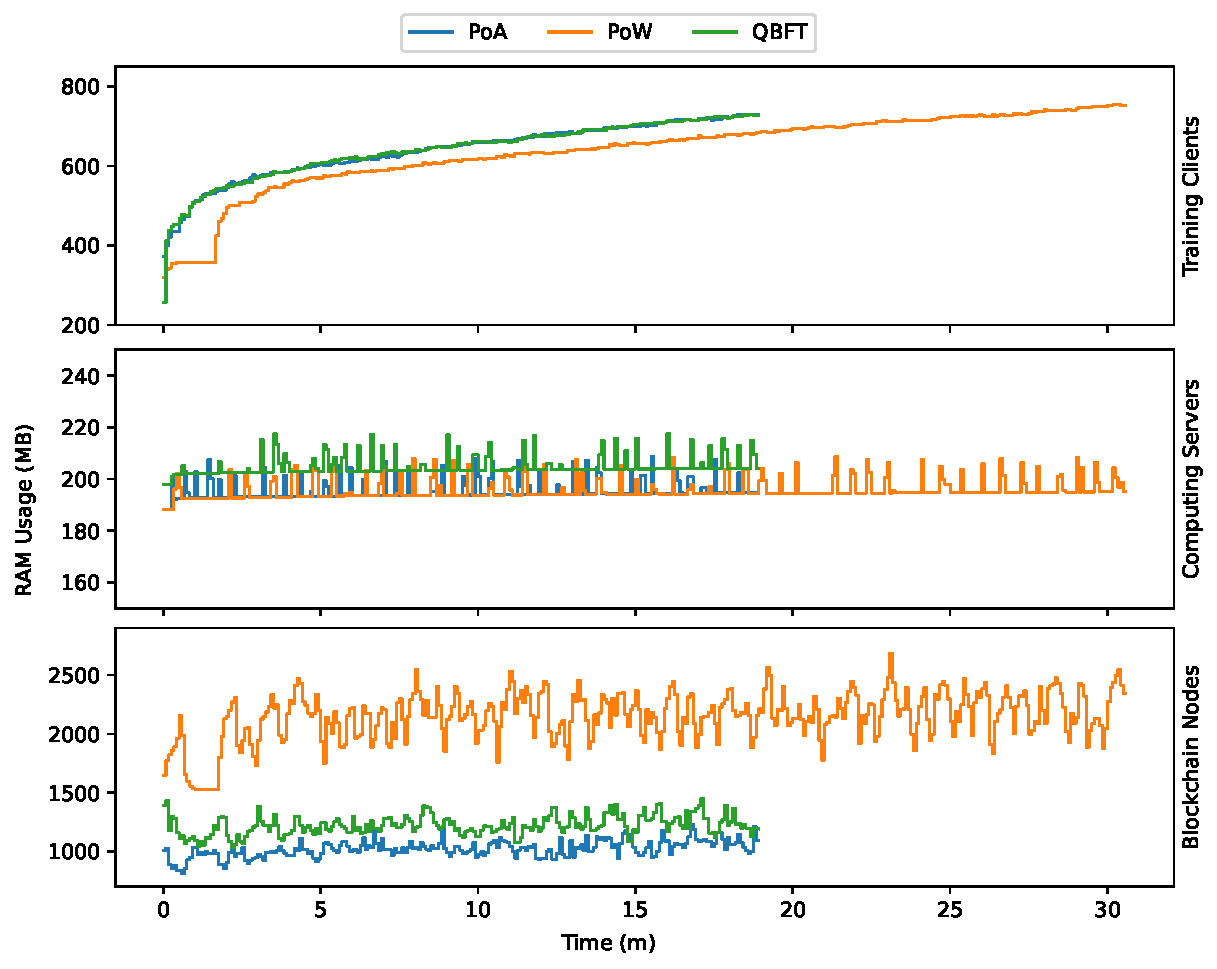
\includegraphics[width=0.8\textwidth]{graphics/01_consensus_ram.pdf}
    \caption{RAM Usage Per Consensus Algorithm}
    \label{fig:ram_consensus_algorithms}
\end{figure}

\begin{figure}[!hpb]
    \centering
    \centering
    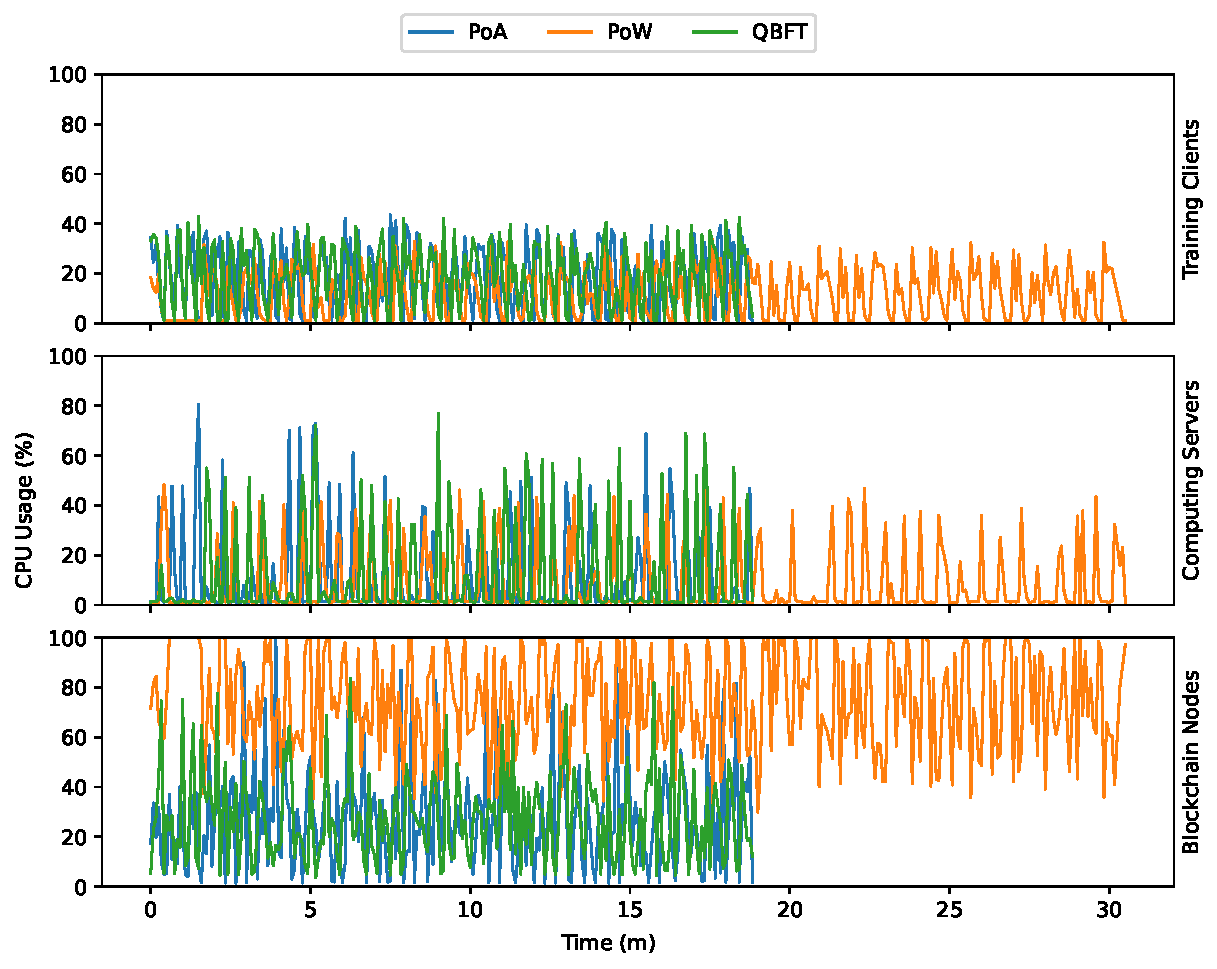
\includegraphics[width=0.8\textwidth]{graphics/01_consensus_cpu.pdf}
    \caption{CPU Usage Per Consensus Algorithm}
    \label{fig:cpu_consensus_algorithms}
\end{figure}

Regarding the clients, the RAM usage and CPU usage do not differ significantly regardless of which consensus algorithm is used. On one hand, we have the RAM usage, where we can observe that the clients reach the same peak. However, the rate at which that peak is reached is different. For PoW, since there are higher transaction latencies, it takes longer to reach the next round, leading to a slower growing RAM usage during the training. On the other hand, we have the CPU usage, where we can observe that there are more idle moments, that is, moments at which the CPU usage is lower. This can also be explained by the higher transaction latencies, during which the clients cannot do anything other than wait.

Regarding the servers, the same reasoning as for the clients can be applied. On one hand, the RAM usage is consistent across different consensus algorithms. We can, however, notice that when using QBFT, the RAM usage at the servers is slightly higher. However, this is a likely negligible difference, as the difference is minimal ($< 10$ MB) considering the total RAM Usage ($\approx 200$ MB). On the other hand, the CPU usage is similar to what we observed for the clients, with a higher amount of idle moments.

Regarding the blockchain nodes, we can visualize a larger difference, both in RAM usage and CPU usage. For both, PoW consumes a much higher level of resources. On average, PoW consumes $2$ times more then RAM and has a $2$ times higher CPU usage. This can also be explained by the way PoW works by solving complex mathematical puzzles, which require intense computation resources.

\section{Conclusions}

In conclusion, we can observe that different consensus algorithms have no direct impact on the accuracy and computation and communication costs at the clients and servers. However, it has an impact on the time and computation and communication costs at the blockchain servers. PoA and QBFT are much faster than PoW. In addition, they require less computation power, both in RAM and CPU. However, QBFT consumes incurs more communication costs than both PoA and PoW. Therefore, there is a clear correlation between the computation costs and the time it takes. The higher the communication costs, the higher the transaction latencies, which translates to slower round times.

Assuming the blockchain network is only being used for Federated Learning, PoA is the most cost-effective of the consensus algorithms we analyzed. In case the network network is needed for other applications, other properties might be required to be taken into account.

For future work, it would be interesting to see if the Ethereum blockchain could be adapted to easily incorporate the custom consensus techniques that were seen in \ref{related_work:consensus_algorithms}. These algorithms work by producing proofs directly from the Machine Learning process. That can lead to better usage of resources if the blockchain network is solely used for a Federated Learning system.